\documentclass[a4paper]{article}
\usepackage[utf8]{inputenc}
\usepackage[russian]{babel}
\usepackage[warn]{mathtext}

\usepackage{graphicx}
\usepackage{wrapfig}
\usepackage{amsmath}
\usepackage{floatflt}
\usepackage{float}
\usepackage{amssymb}
\usepackage{mathrsfs}

\usepackage{longtable}
\usepackage{multicol}
\usepackage{multirow}

\usepackage{lscape}
\usepackage{hvfloat}

\usepackage{indentfirst}

\usepackage[left=15mm, top=20mm, right=15mm, bottom=20mm, footskip=10mm]{geometry}
\linespread{1.3}
\usepackage{multicol}

\graphicspath{ {pics/} }

\begin{document}
\begin{titlepage}
\noindent

	\centering
	\vspace{2cm}
	{\scshape\LARGE Московский физико-технический институт (НИУ)\par}
	\vspace{1cm}
	{\scshape\Large Лабораторная работа\par}
	\vspace{1cm}
	{\huge\bfseries Твердотельный лазер на YAG:Nd$^{3+}$ \par}
	\vspace{1cm}

	%\vspace{0.5cm}
	\vfill
	
\begin{flushright}
	{\large выполнили студенты 4-ого курса ФЭФМ}\par
	\vspace{0.3cm}
	{\LARGE Анисимов Михаил, Б04-855} \par
	{\LARGE Водзяновский Яромир, Б04-855} \par
	{\LARGE Атепалихин Артемий, Б04-855} \par
	{\LARGE Трушин Александр, Б04-852} \par
	{\LARGE Рудоманова Полина, Б04-853} \par
	\vspace{0.3cm}
	{\large преподаватель}\par
	\vspace{0.3cm}
	{\LARGE Юрий Юрьевич Брославец} \par
\end{flushright}

\vfill

% Bottom of the page
	Долгопрудный, 2020 г.
\end{titlepage}

\tableofcontents

\newpage

\section{Теория}
\subsection{Инверсия активной среды как необходимое условие генерации лазера}

Если для плотности инверсной заселености $N = n_2 - (g_2/g_1) n_1$. Выполняется условие:

\begin{equation}
	N > 0
\end{equation}

Очевидно, что в состоянии термодинамиеского равновесия  инверсная заселенность - отрицательная. Коэфицент усиления $\chi_1$ пространственно-однородной среды описывается выражением:

\begin{equation}
	\chi_1 = \sigma N
\end{equation}

где $\sigma$ - сечение вынужденных переходов между рабочими уровнями. Для создания и поддержания инверсии применяют тот или иной способ возбуждения (или, как говорят, способ накачки) активной среды. Активная среда лазера характеризуется линейным коэфицентом оптического усиления $\chi_1$ и линейным коэфицентом поглощения на неактивных центрах и рассеяния $\chi_2$. Распостранение светого потока в активной среде описывается законом Бугера:

\begin{equation}
\label{Buger}
	dS_\omega = [\chi_1(z) - \chi_2] S_\omega (z)dz
\end{equation}

Для практического получения режима генерации необходимо ввести положительную обратную связь. В лазере обратуню связь обычно осуществляют размещением активной среды между двумя зеркалами (например, между плоскопараллельными зеркалами). Если потери в резонаторе определяются только пропусканием зеркал, то порог генерации будет достигнут при выпонении условия (очевидно следует из \ref{Buger} ):

\begin{equation}
	R_1 R_2 \exp(2 \sigma (n_2-n_1) L) = 1
\end{equation}

\subsection{Условия стационарной генерации}

Пусть $L$-длина активной среды. Используя \ref{Buger} находим:

\begin{equation}
	\ln\frac{S(L)}{S(0)} = \int_0^L[\chi_1(z)-\chi_2]dz
\end{equation}

Для упращения будем использовать среднее по длине значение коэфицента усиления:

\begin{equation}
	S(L) = S(0) \exp(L[ <\chi_1> - \chi_2 ]) = S(0)T
\end{equation}

Если у левого зеркала интенсивность излучения $S(0)$, то после прохода резонатора у правого зеркала  будем иметь $TS(0)$. После отражения от правого зеркала и повторного прохода резонатора + отражения от левого зеркала получим мощность $R_1 R_2 T^2 S(0)$, которая в силу стационарности должна равняться $S(0)$ отсюда имеем:

\begin{equation}
	< \chi_1 > = \chi_2 + \frac{1}{2L}\ln(\frac{1}{R_1R_2})
\end{equation}

Это и есть условие стационарной генерации.

\subsection{Получение инверсной населенности с помощью оптической накачки}

Различают некогерентную и когерентную оптические накачки. При некогерентной накачке используется некогерентное накачивающее излучение, его источником могут служить газоразрядные импульсные лампы, лампы непрерывного горения (газоразрядные и накаливания), искровые разрядники, пламя и т.д. При когерентной накачке источником накачивающего излучения служит вспомогательный лазер. Для оптической накачки характерна возможность осуществления исключительно высокой селективности возбуждения.
Специфика оптической наакачки проявляется и в том, что она всегда индуцирует в канале вобуждения обратный процесс, имеющий примерно такую же вероятность что и прямой процесс, связанный с поглощением излученя. Отнесенная к единице времени вероятность поглошения накачки:

\begin{equation}
	W_p  = B \rho_p(\nu) 
\end{equation}

Наряду с поглощением происходит обратный процесс - стимулированное испускание, индуцированное излучением накачки. Вероятность этого процесса:

\begin{equation}
	W_p' = B' \rho_p(\nu)
\end{equation}

При этом справедливо соотношение Эйнштейна:

\begin{equation}
	gB = g'B'
\end{equation}

Существование двух встречных процессов запрещает совмещать каналы возбуждения и генерации при оптической накачке. Отсюда, в частности следует что минимально необходимое число уровней активного центра при оптической накачке - три.

\subsection{Формирование поля излучения в резонаторе лазера}

\subsubsection{Резонасные частоты}

Приведем общеизвестную формулу для резонансных частот в прямоугольном резонаторе:

\begin{equation}
	\nu_q = q \frac{c}{2Ln}
\end{equation}

В такой упрощенной моделе спектр - эквидистантный $\Delta \omega ' = \frac{\pi c}{Ln}$. Полное число мод - $M = \Delta \omega / \Delta \omega'$ Это число растет с увеличением оптической длины резонатора и ширины линии усиления. Введем добротность резонатора : $Q = \omega_0 / \Delta \omega_\Gamma$, где $\omega_\Gamma$ - ширина спектрального пика. Для разрешения спектральных пиков необходимо выполнение условия: $\Delta \omega_\Gamma < \Delta \omega '$. В частности используя время жизни фотона для двухзеркального резонатора:

\begin{equation}
	\tau_c = - \frac{2L}{c \ln(R_1 R_2 (1-T)^2)}
\end{equation}

Можно получить критерий $1/\tau_c <  \frac{\pi c}{Ln}$. Для ширин лини генерации лазера приводится следующее соотношение:

\begin{equation}
	\delta \nu = \frac{2 \pi (\Delta \nu_c)^2 \hbar \omega}{P^{(0)}}
\end{equation}

где $P^{(0)}$ - мощность генерации лазера

\subsubsection{Моды оптического резонаора}

Каждый тип попречной моды имеет определенную структуру светового пятна на зеркале резонатора. В декартовоой системе координат рспределение поля можно описать с помощью ф-ций Эрмита и Гаусса:

\begin{equation}
	u_{mn}(x, y) = A_0 H_m(\sqrt{2}\frac{x}{\omega}) H_n(\sqrt{2}\frac{y}{\omega}) \exp{(-i \frac{k(x^2+y^2)}{2q})}
\end{equation}

Где $\frac{1}{q} = \frac{1}{R} - i \frac{\lambda}{\pi \omega^2}$

\subsection{Режимы работы лазеров}
\subsubsection{Режим свободной генерации}
Предположим, что в резонаторе лазера находится только активный элемет и нет каких-либо нелинейных элементов или элементов, свойства которых меняются под воздействием внешних параметров. Наиболее интересна картина свободной генерации в твердотельных лазерах. Излучение лазера в этом режиме представляет из себя последовательность относительно коротких импульсов или, как принято говорить, пичков. Длительность отдельного пичка рвана $10^{-7}-10^{-6}$ с, мощность достигает значений $10^4 - 10^5$ Вт. Природа пичков до сих остается предметом иследований, на основе одномодовой модели можно показать, что регулярные затухающие пульсации связаны с переходными процессами, сопровождающими начало генерации при появлении имплульса накачки.

\subsubsection{Режим генерации гиганских импульсов} % (fold)

Управляя добротностью резонатора, сначала обеспеечивают высокий уровень вредных потерь, т.е. специльно поднимают порог генерации. Это позволяет создать значительную инверсную заселенность в активной среде. Затем по сигналу извне уровень потерь понижают до минимально возможного значения, в результате чего начальная инверсная заселенность оказывается существенно выше пороговой. В этих условиях вместо последовательности пичков высвечивается единичный короткий световой импульс большой мощности (так называемый гигантский импульс). Мощность гигантского импульса тем больше, чем значительнее первышение начальной инверсной заселенности над пороговым значением инверсной заселенности. Мощность получаемых на практике гигантских импульсов достигает $10^9$ Вт. Дальнейшему росту импульса препятсвуют спонтанное излучение и сверхлюминесценсия. Длительность гиигансткого импульса имеет порядок $10-100$ нс. Для реализации в резонатор помещают модулятор, управляемый внешним сигналом. Обычно он работает как "оптический затвор"

\subsubsection{Режим генерации гиганстких импульсов при пассивной модуляции добротности} % (fold)

Пассивная модуляция добротности основана на применении нелинейных элементов. Широко используются просветляющие фильтры - оптические затворы, работающие на основе нелинейного явления просветления среды. Как и при активной модуляции добротности, процесс формирования состоит из двух этапов: медленного линейнго развития и быстрого нелинейного развития. Просветляющий фильтра представляет собой нелинейный резонансный поглоитетель, спосбный обратимо имзенить коэфицент поглощения под действием некоторой достаточно большой интенсивности потока. В качестве просветляющих сред часто используются растворы органических красителей - цианиновых и полиметинновых.

\subsection{Динамика генерации лазера в различных режимах работы} % (fold)
\label{sub:динамика_генерации_лазера_в_различных_режимах_работы}

\subsubsection{Система уравнений, описывающая динамику генерации лазера}

Рассмотрим четырехуровневую схему. Считая, что переходы между уровнями 4 и 3 и уровнями 2 и 1 являются быстрыми, можно положить $n_4 \approx n_2 \approx 0$. В этом случае скоростные уравнения можно записать следующим образом:

\begin{equation}
\begin{cases}
\frac{dn_3}{dt} = W_pn_1 - Bqn_3 - \frac{n_3}{\tau} \\
\frac{dq}{dt} = V_a Bqn_3 - \frac{q}{\tau_c} \\
n_1 + n_3 = N_t
\end{cases}
\end{equation}

Вводя инверсную заселенность ;$N = n_3 - n_2 \approx n_3$ можно переписать в виде:

\begin{equation}
\begin{cases}
\label{main_cases}
\frac{dN}{dt} = W_p(N_t - N) - BqN -- \frac{N}{\tau} \\
\frac{dq}{dt} = (BV_aN - \frac{1}{\tau_c})q
\end{cases}
\end{equation}

\subsubsection{Работа четырехуровневого лазера в непрерывном режиме}

Рассмотрим работу лазера при стационарной накачке. Поскольку такая накачка приводит к стационарному режиму генерации, в этом случае режим работы лазера можно рассматривать как непрерывный.

Определим пороговое условие генерации лазера. Предположим, что в момент времени $t=0$ в резонаторе вследствие спонтанного испускания присутвует некоторое небольшое число фотонов $q$. При этом из (\ref{main_cases}) для того, чтобы $\frac{dq}{dt} > 0$, нужно чтобы $(V_a BN - 1/\tau_c) > 0$/ В этом случае генерация возикает, если инверсия населенностей $N$ достигает некоторого критического значения $N_c$, определяемого выражением

\begin{equation}
	N_c = \frac{1}{V_a B \tau_c} = \frac{\gamma}{\sigma l}
\end{equation}

где $\gamma$ - суммарные потери в резонаторе за проход в одном направлении, $\sigma$ - сечение перехода генерации. Таким образом, критическая (пороговая) скорость накачки соответствует ситуации, когда полная скорость накачки уровней $W_{\text{ср}}(N_t - N_c)$ уравновешивает скорость $N_c / \tau$ спонтанных переходов с рабочего уровня:

\begin{equation}
	W_{cp} = \frac{N_c}{(N_t - N_c) \tau}
\end{equation}

Если $W_p > W_{cp}$, то число фотонов $q$ будет возрастать от начальной величины, определяемой спонтанным излучением, и если $W_p$ не зависит от времени, то в конце концов достигнет некоторого постоянного значения $q_0$. Это стационарное значение и соответсвующее ему стационарное значение инверсии $N_0$ получаются из уравнений (\ref{main_cases}) если $\dot{N} = \dot{q} = 0$

\begin{equation}
\begin{cases}

N_0 = \frac{1}{V_a B \tau_c} = N_c \\
q_0 = V_a \tau_c [W_p(N_t - N_0) - \frac{N_0}{\tau}]

\end{cases}
\end{equation}

Также можно выразить:

\begin{equation}
	B = \frac{\sigma l c}{V_a L'} = \frac{\sigma c}{V}, \; \; \tau_c = \frac{L'}{c \gamma}
\end{equation}

\subsubsection{Работа лазера в нестационнарных режимах генерации при ступенчатом включении импульса накачки}

Рассмотрим работу лазера при нестационарной накачке, которая описывается ступенчатой ф-цией. Для данной временной зависимости скорость накачки имеет следующую временную зависимость: $W_p = 0$ при $t < 0$ и $W_p(t) = W_p$ при $t>0$. При небольших колебаниях инверсии и кол-ва фотонов можно записать:

\begin{equation}
	\begin{cases}
		N(t) = N_0 + \delta N \\
		q(t) = q_0 + \delta q
	\end{cases}
\end{equation}

Тогда с учетом малости изменения из (\ref{main_cases}) можно получить:

\begin{equation}
	\begin{cases}
		\delta \dot{N} = - \delta N(W_p + \frac{1}{\tau}) - B(q_0 \delta N + N_0 \delta q) \\
		\delta \dot{q} = Bq_0 V_a \delta N
	\end{cases}
\end{equation}

Отсюда получим уравнение колебаний, решение которого будет:

\begin{equation}
	\delta q = \delta q_0 \exp(st),, \; \; s = -1/t_0 \pm[(1/t_0)^2 - \omega^2]^{1/2}
\end{equation}

При $1/t_0 < \omega$ решение будет представлять из себя затухающие колебания

\subsubsection{Особенности генерации в режиме модуляции добротности}

В режиме модуляции добротности лазер позволяет получать генерацию в виде импульсов с малой длительностью и высокой пиковой мощностью (гигантские импульсы). В случае если резонатор имеет низкую добротность, когда модулятор перекрывает излучение, можно считать, что $q = 0$, поэтому из (\ref{main_cases}) получаем уравнение:

\begin{equation}
	\frac{dN}{dt} = W_p (N_t-N) - N/\tau
\end{equation}

Сделаем замену $x = W_p (N_t - N) - N/\tau$, $dx = - (W_p + \frac{1}{\tau})dN$. В реузльтате получим уравнение:

\begin{equation}
	\frac{dx}{dt} = - x(W_p + \frac{1}{\tau})
\end{equation}

Далее решая его и подставляя н/у, получим:

\begin{equation}
	N = \frac{W_p N_t}{W_p + \frac{1}{\tau}}[1-\exp(-(W_p + \frac{1}{\tau})t)]
\end{equation}

При длительной накачки инверсия приближается к стационраному значению, практически линейно зависящему от уровня накачки.

При высокой добротности резонатора - индуцированные переходы преобладают над спонтанными, упрощая досновную систему (\ref{main_cases}), находим положение максимума генерации:

\begin{equation}
	N = N_c = \frac{1}{V_a B \tau_c}
\end{equation}

А для количества фотонов имеем:

\begin{equation}
	q = V_a(N_c \ln(N/N_0)+N_0 - N)
\end{equation}

\newpage



\section{Экспериментальная часть}
\subsection{Режим свободной генерации}

Исследуем зависимость выходной мощности от мощности накачки. Для этого сперва снимем напряжение, поступающее на конденсатор ёмкостью $100 \; \text{мкФ}$ и воспользуемся известной формулой, чтобы найти энергию зарядки конедсатора. Энергию излучения получим через известную пиковую мощность и длительность импульса

\begin{figure}[h]
\centering
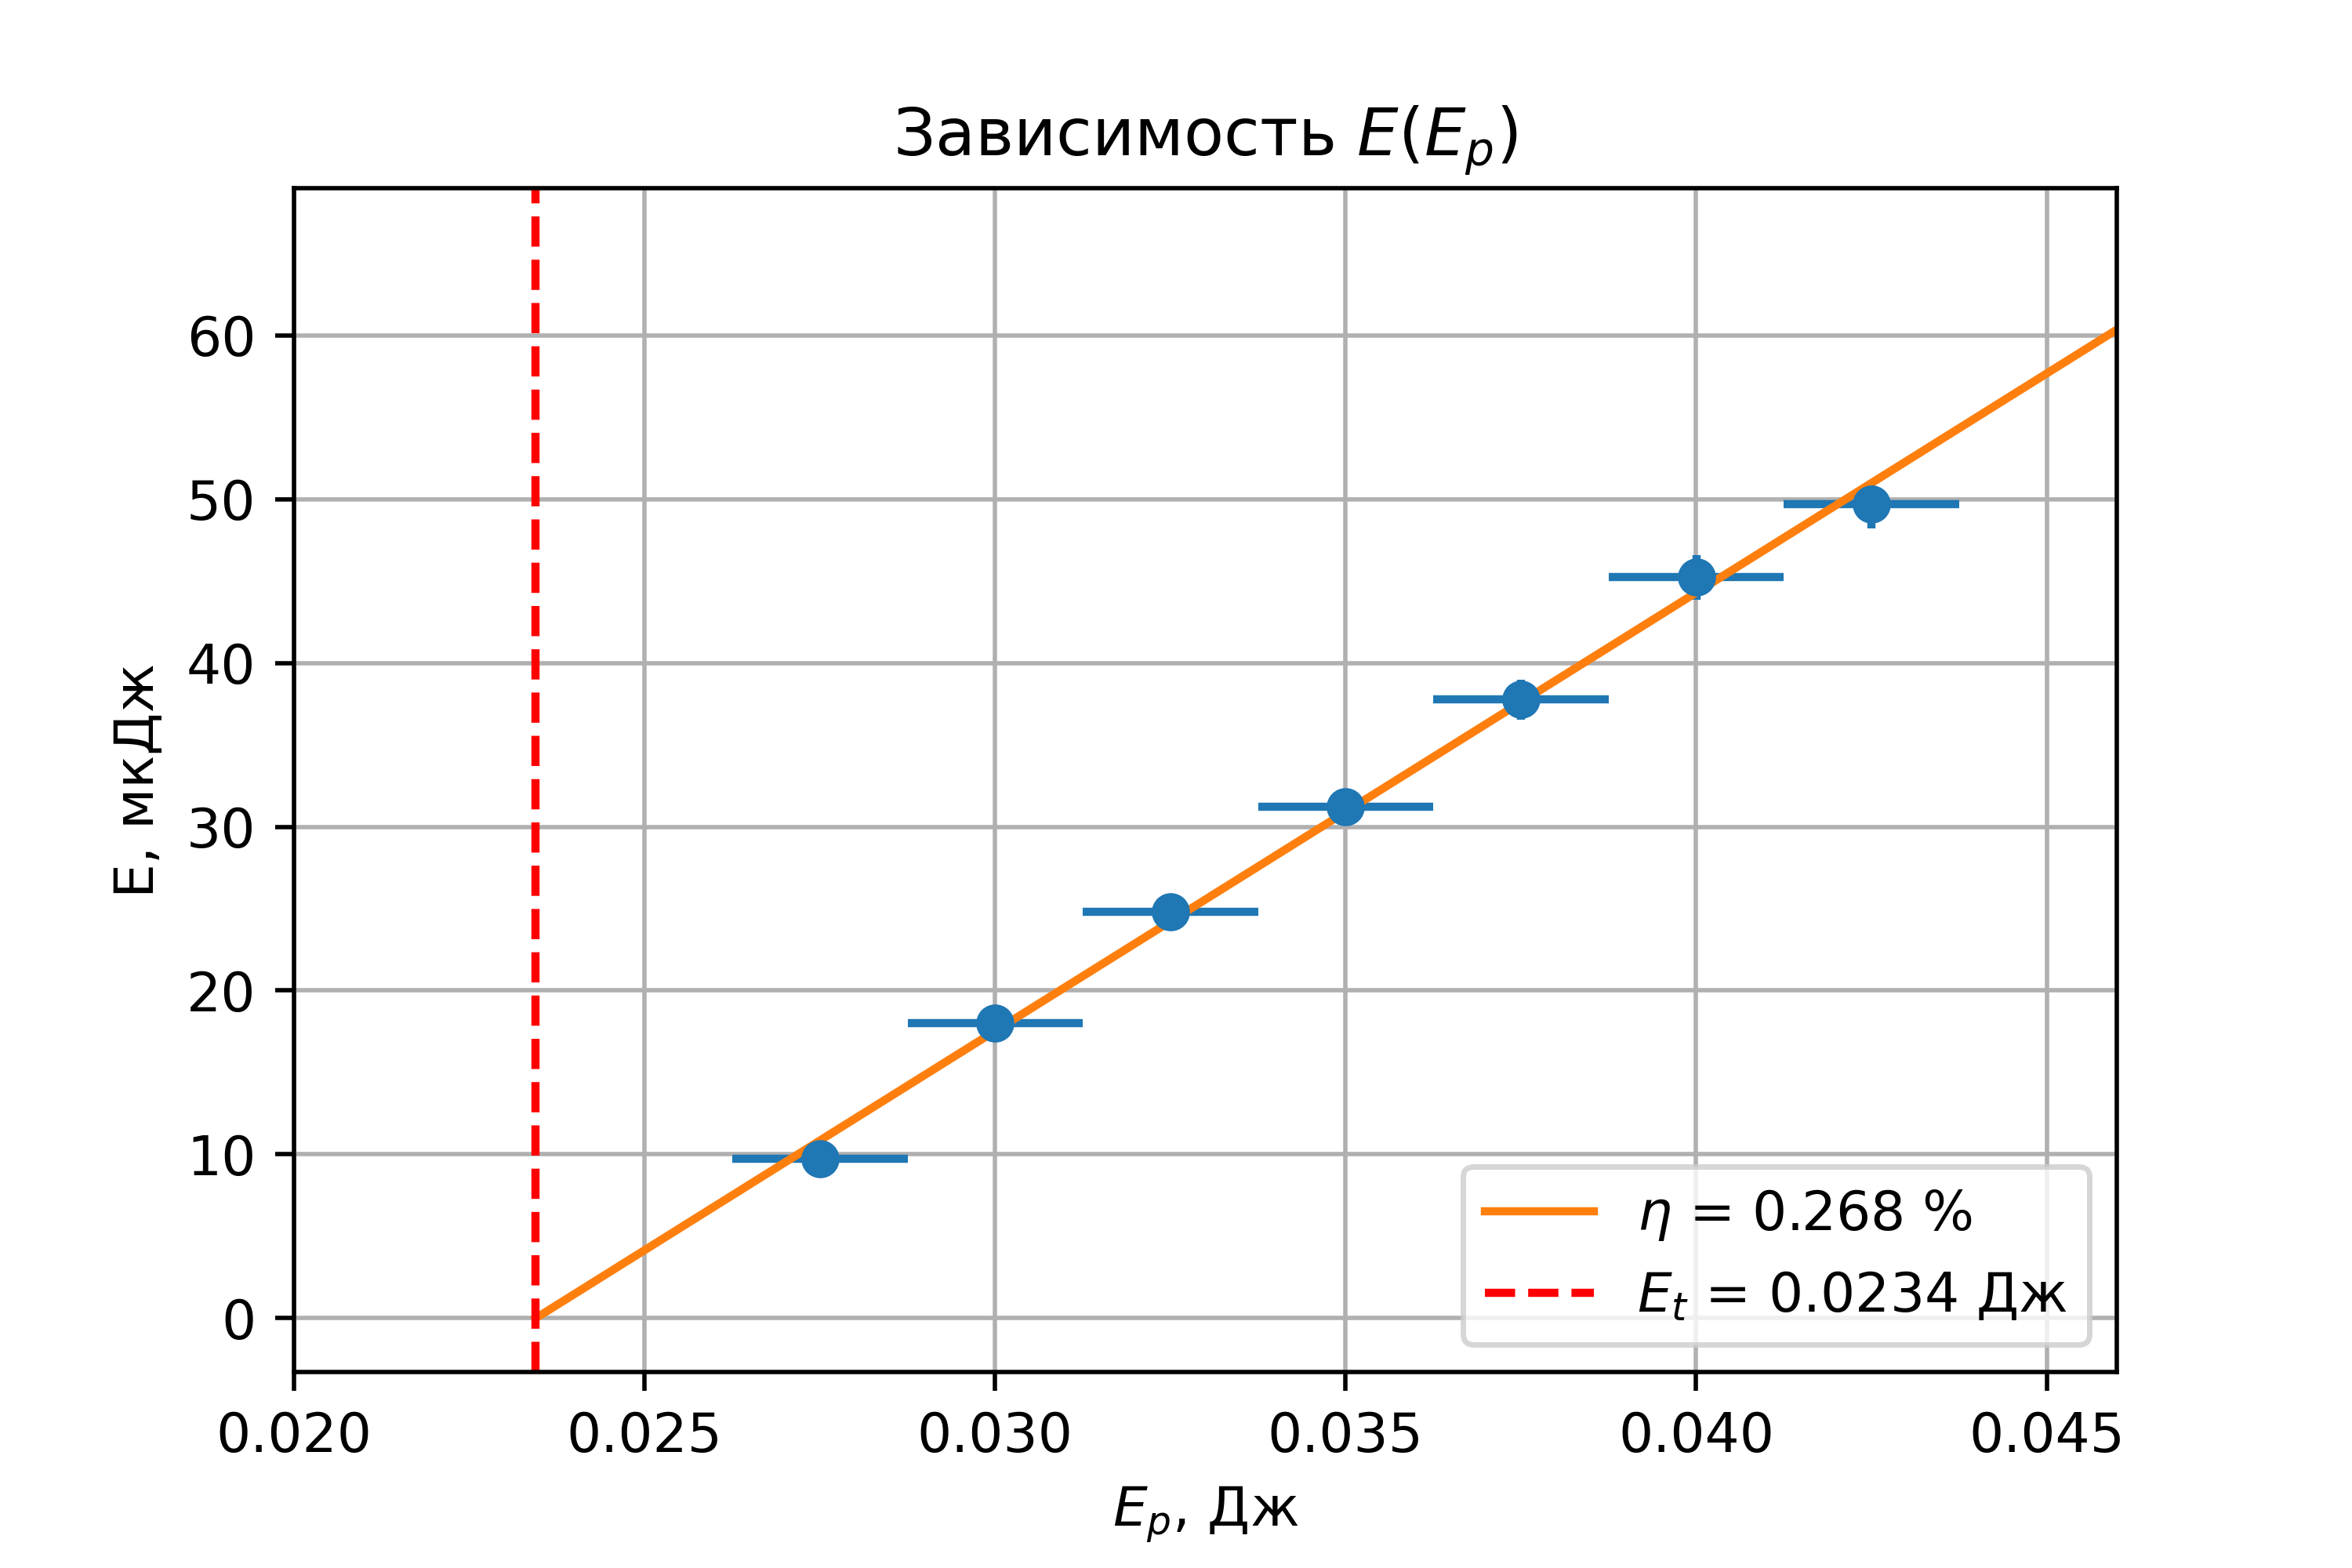
\includegraphics[width=0.65\linewidth]{linear_W1.png}
\caption{Зависимость энергии излучения от энергии накачки}
\label{fig:graph}
\end{figure}

Отсюда получим КПД и пороге генерации: 

\begin{equation*}
	\eta = 0.268 \pm 0.007 \; \%
\end{equation*}

\begin{equation*}
	E_t = 0.0234 \pm 0.0003 \; \text{Дж}
\end{equation*}

Дополнительно снимем зависимость длительности импульса от энергии накачки. Снятая зависимость получилась немонотонной:

\begin{figure}[h]
\centering
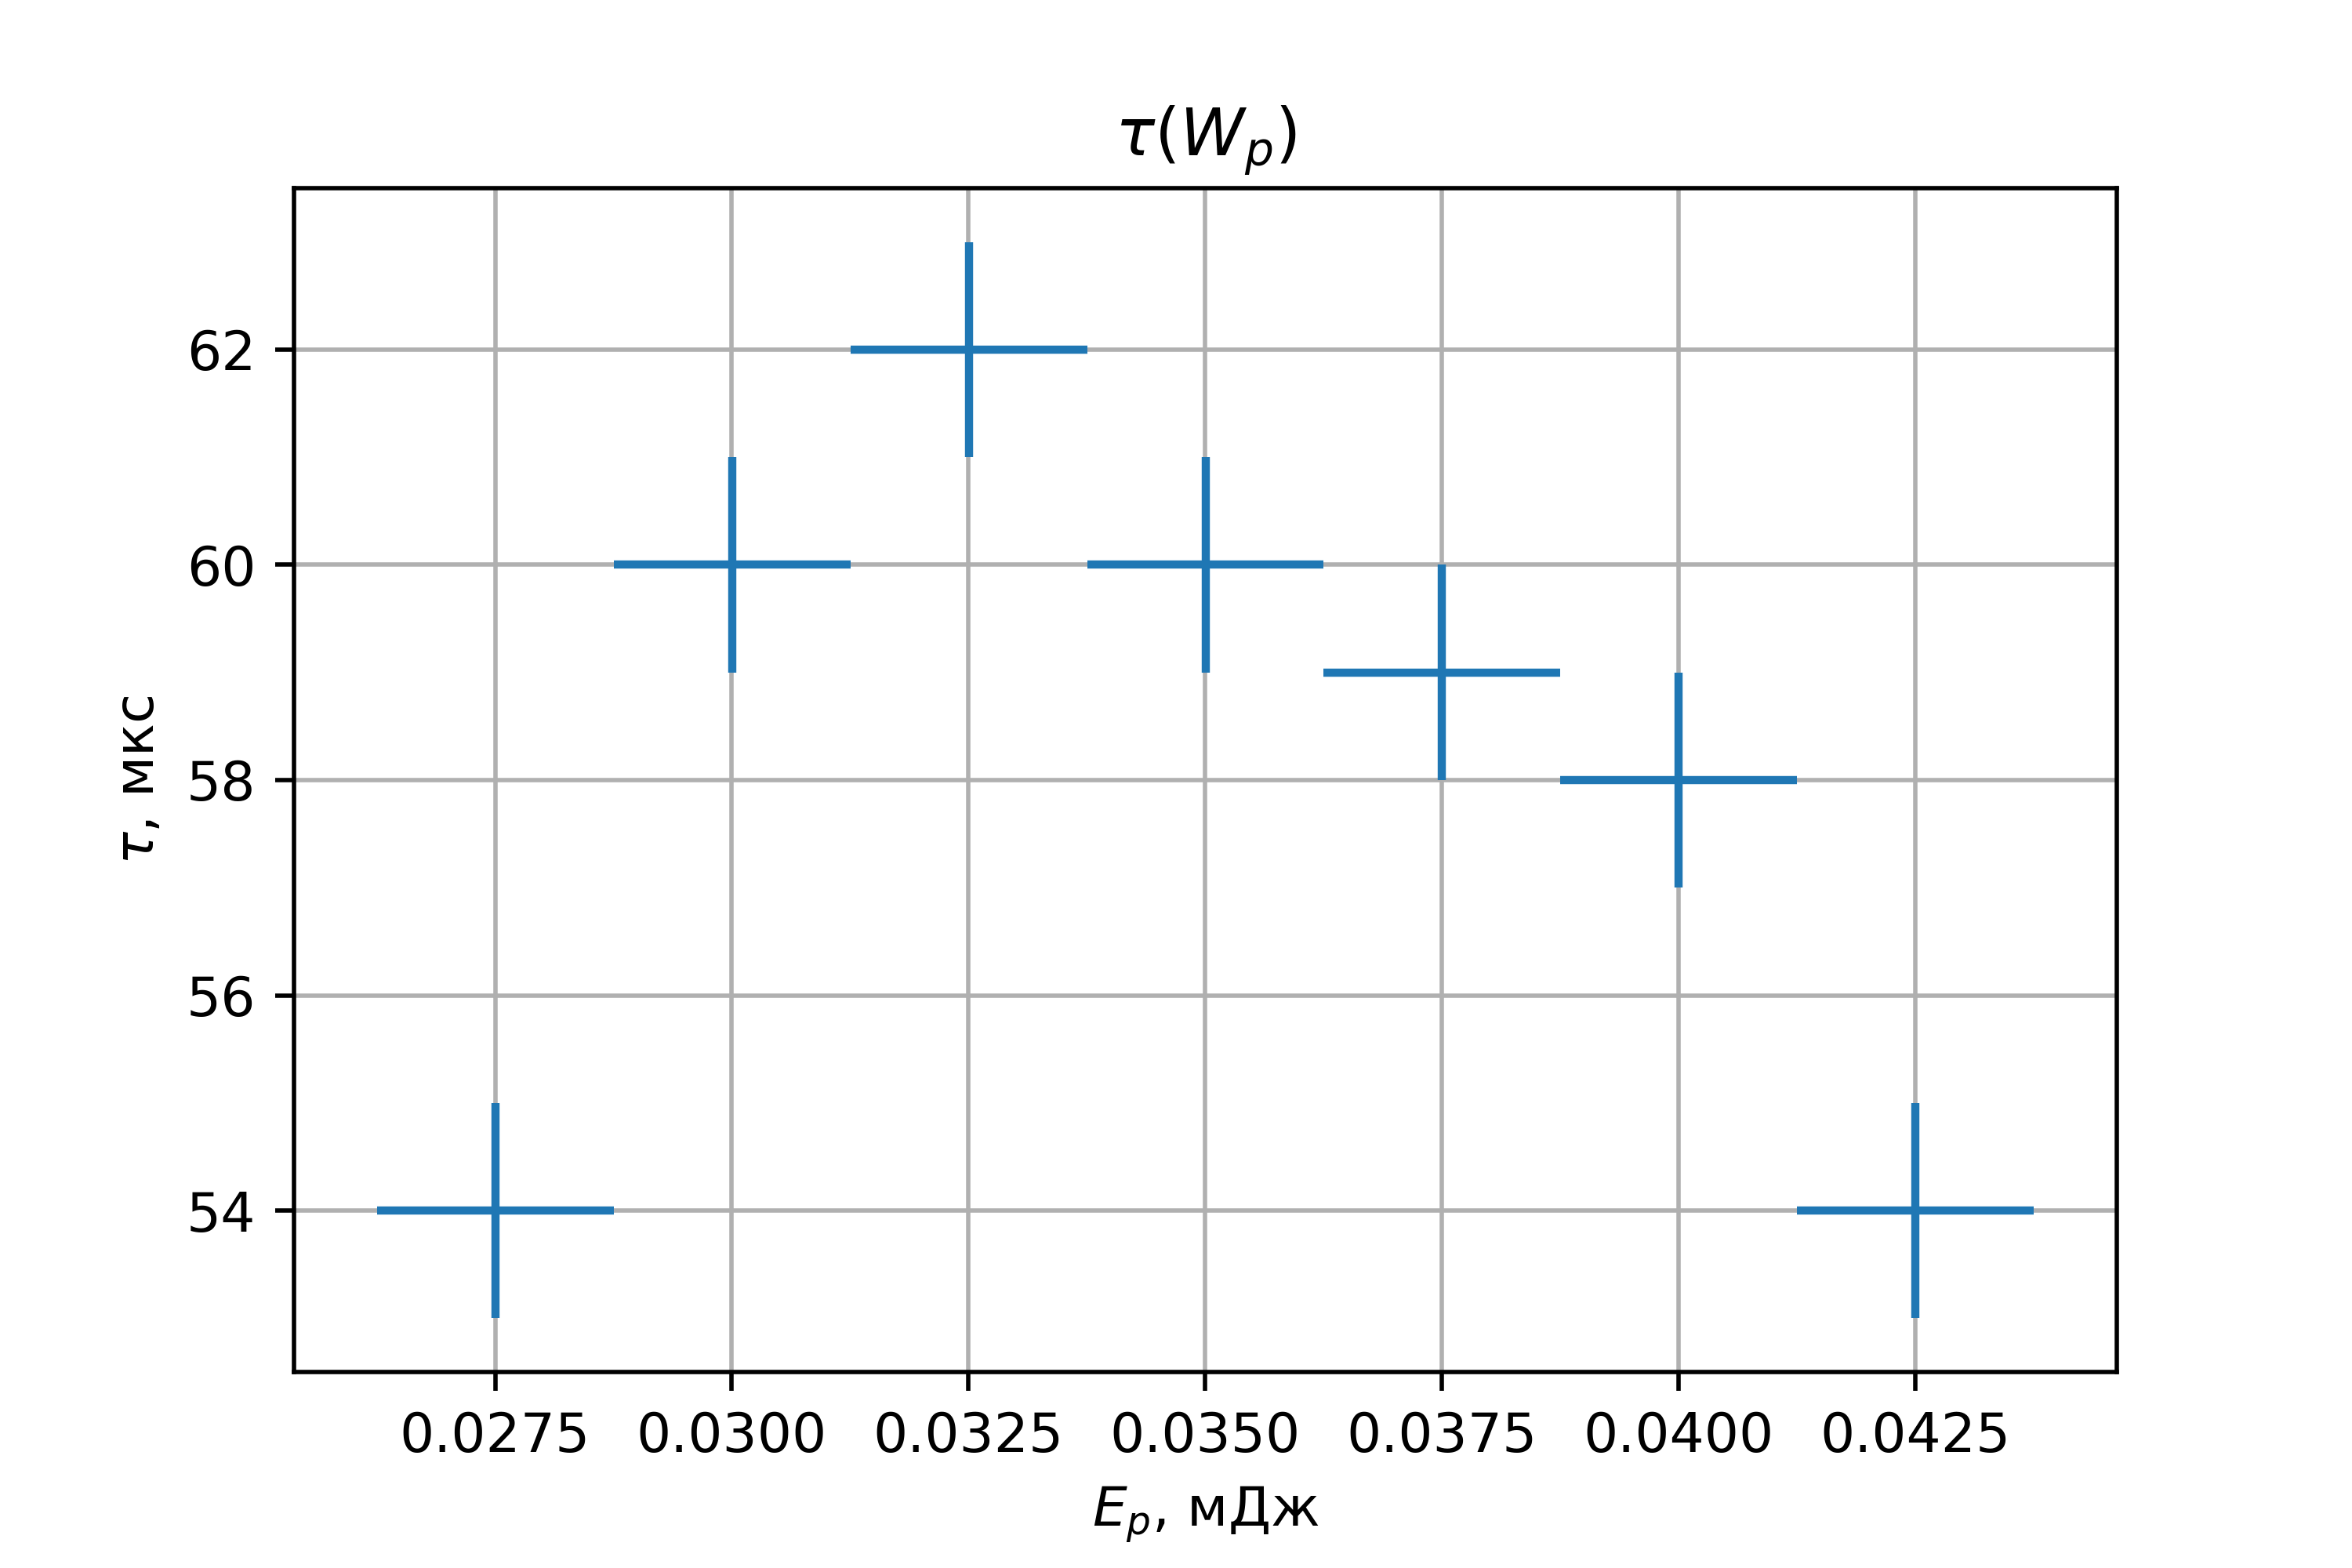
\includegraphics[width=0.65\linewidth]{linear_width1.png}
\caption{Зависимость длительности импульса от энерги накачки}
\label{fig:graph}
\end{figure}

\newpage

\subsection{Режим модуляции добротности}

Далее, пользуясь фотофильтром снимем ту же зависимость в режиме модуляции добротности

\begin{figure}[h]
\centering
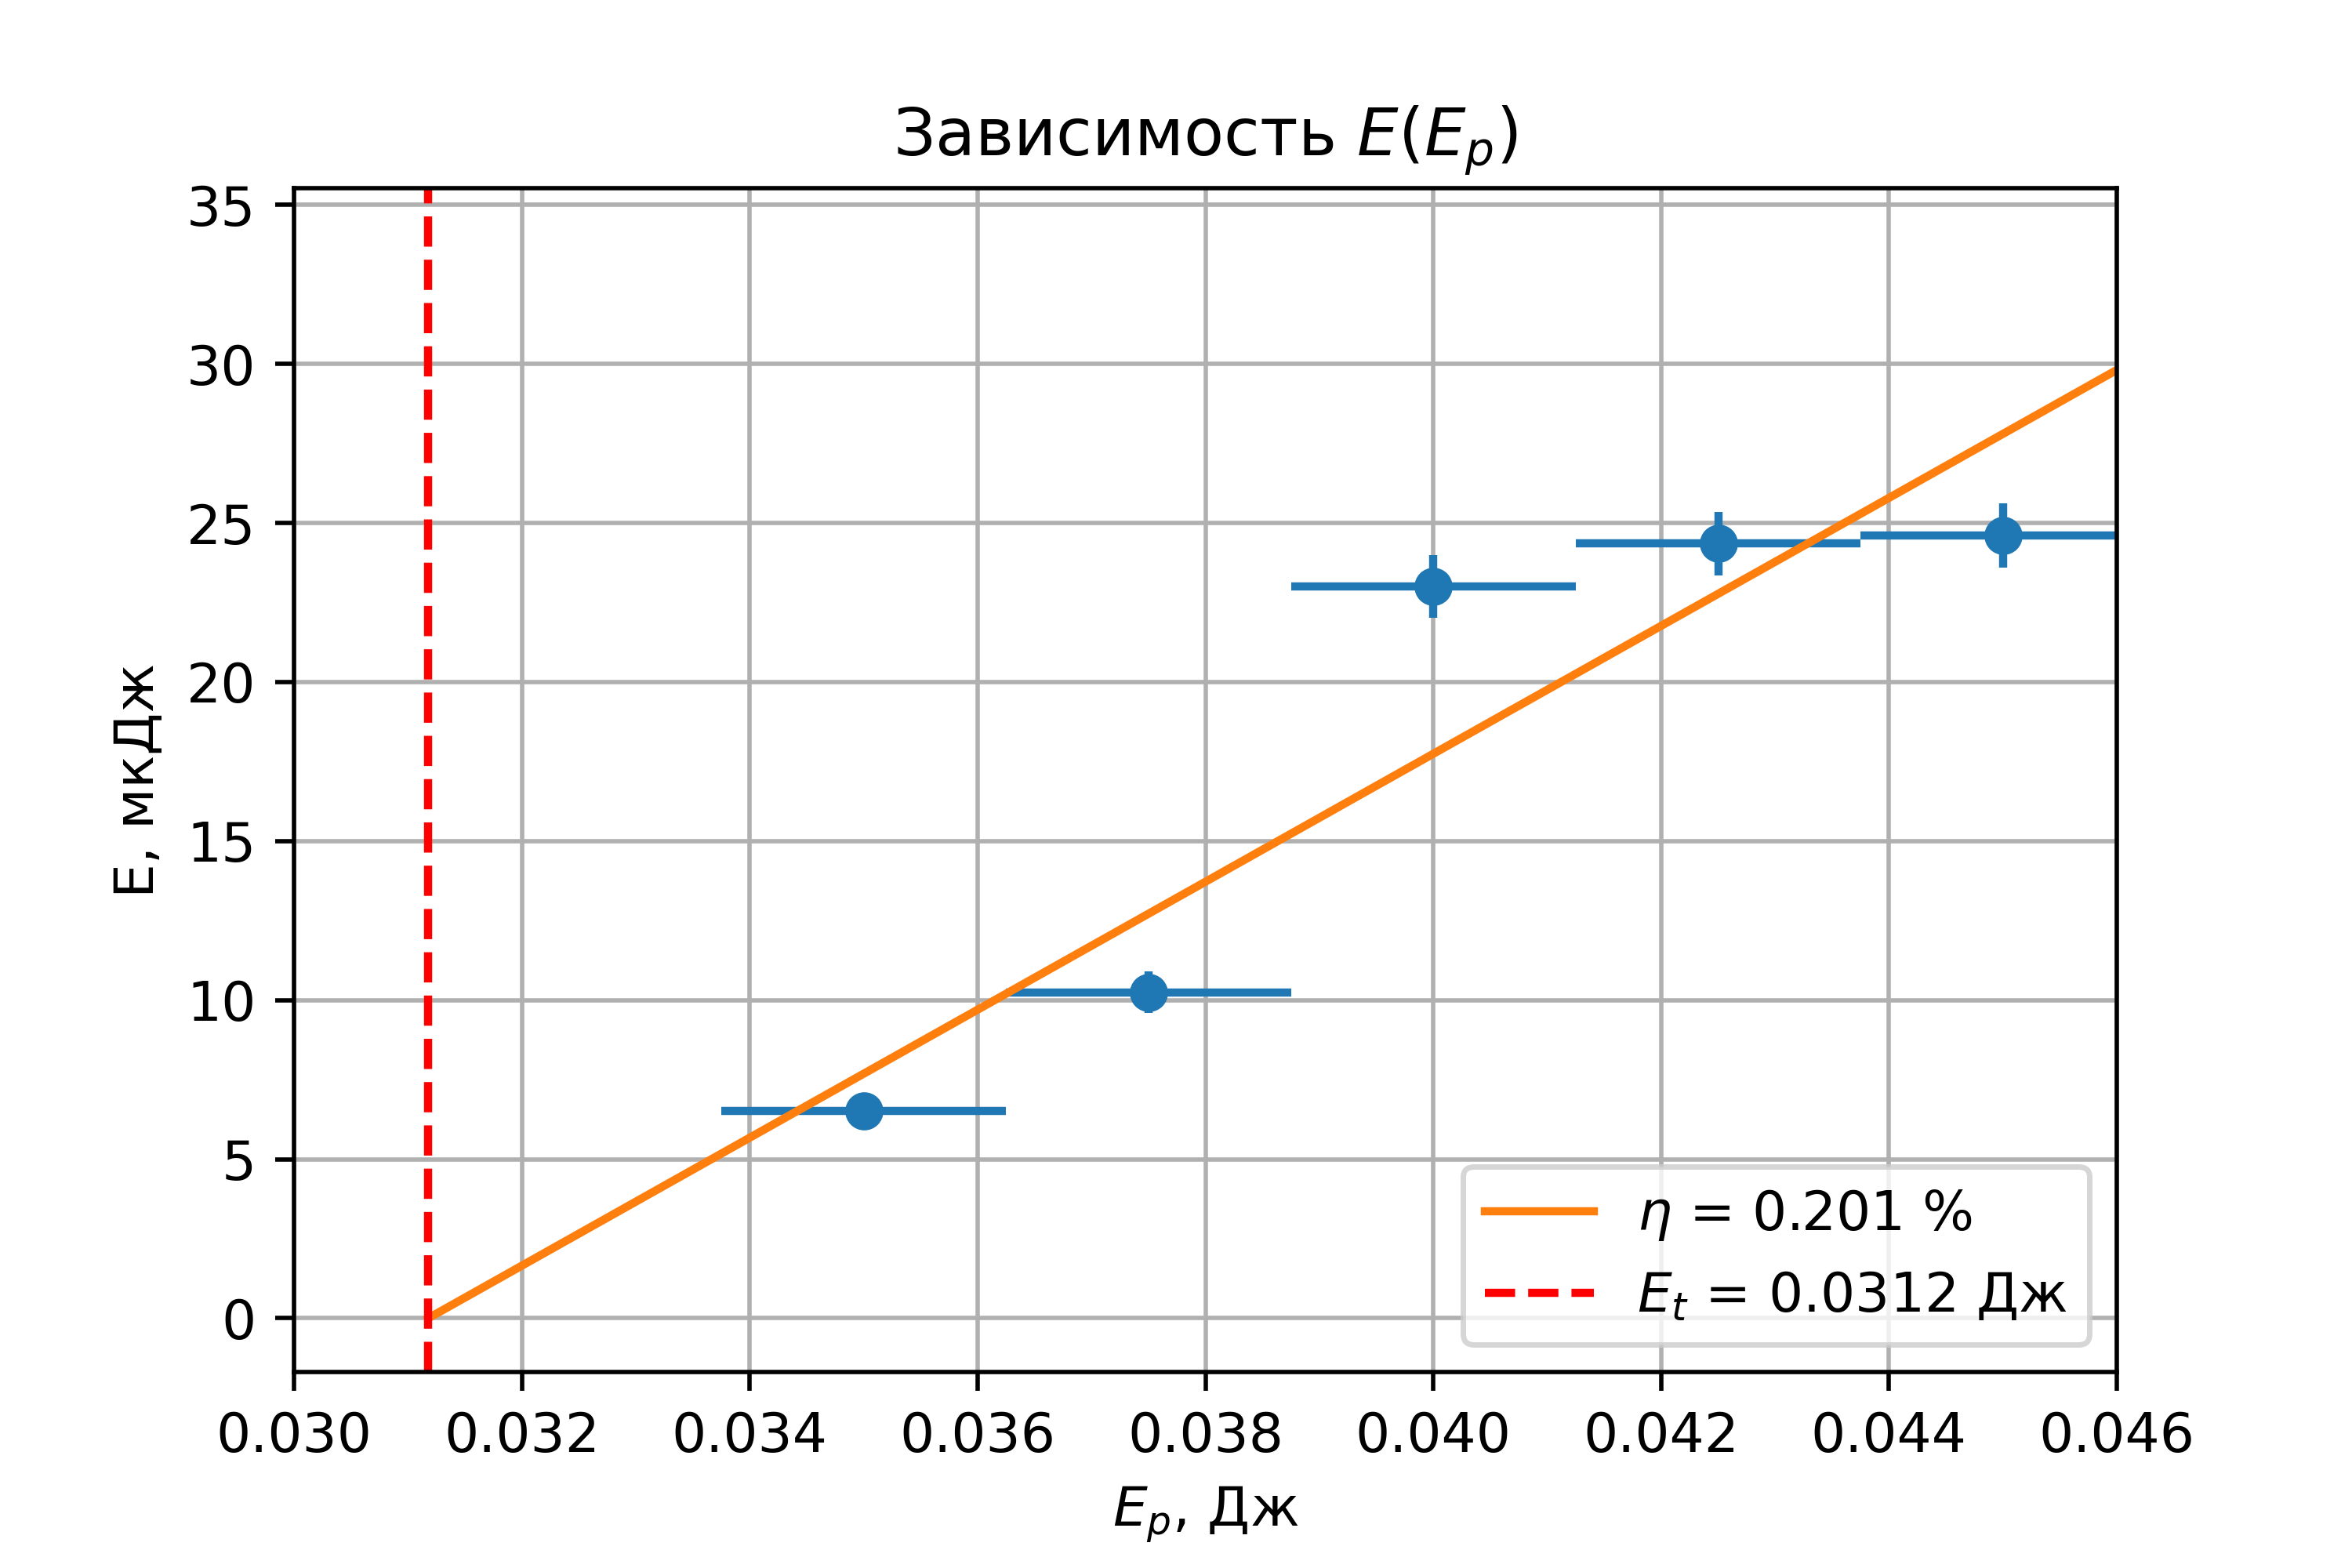
\includegraphics[width=0.65\linewidth]{linear_W2.png}
\caption{Зависимость энергии излучения от энергии накачки}
\label{fig:graph}
\end{figure}

Отсюда получим КПД и порог генерации: 

\begin{equation*}
	\eta = 0.20 \pm 0.05 \; \%
\end{equation*}

\begin{equation*}
	E_t = 0.0312 \pm 0.0023 \; \text{Дж}
\end{equation*}

И снова зависимость длительности импульса не имеет конкретного характера:

\begin{figure}[h]
\centering
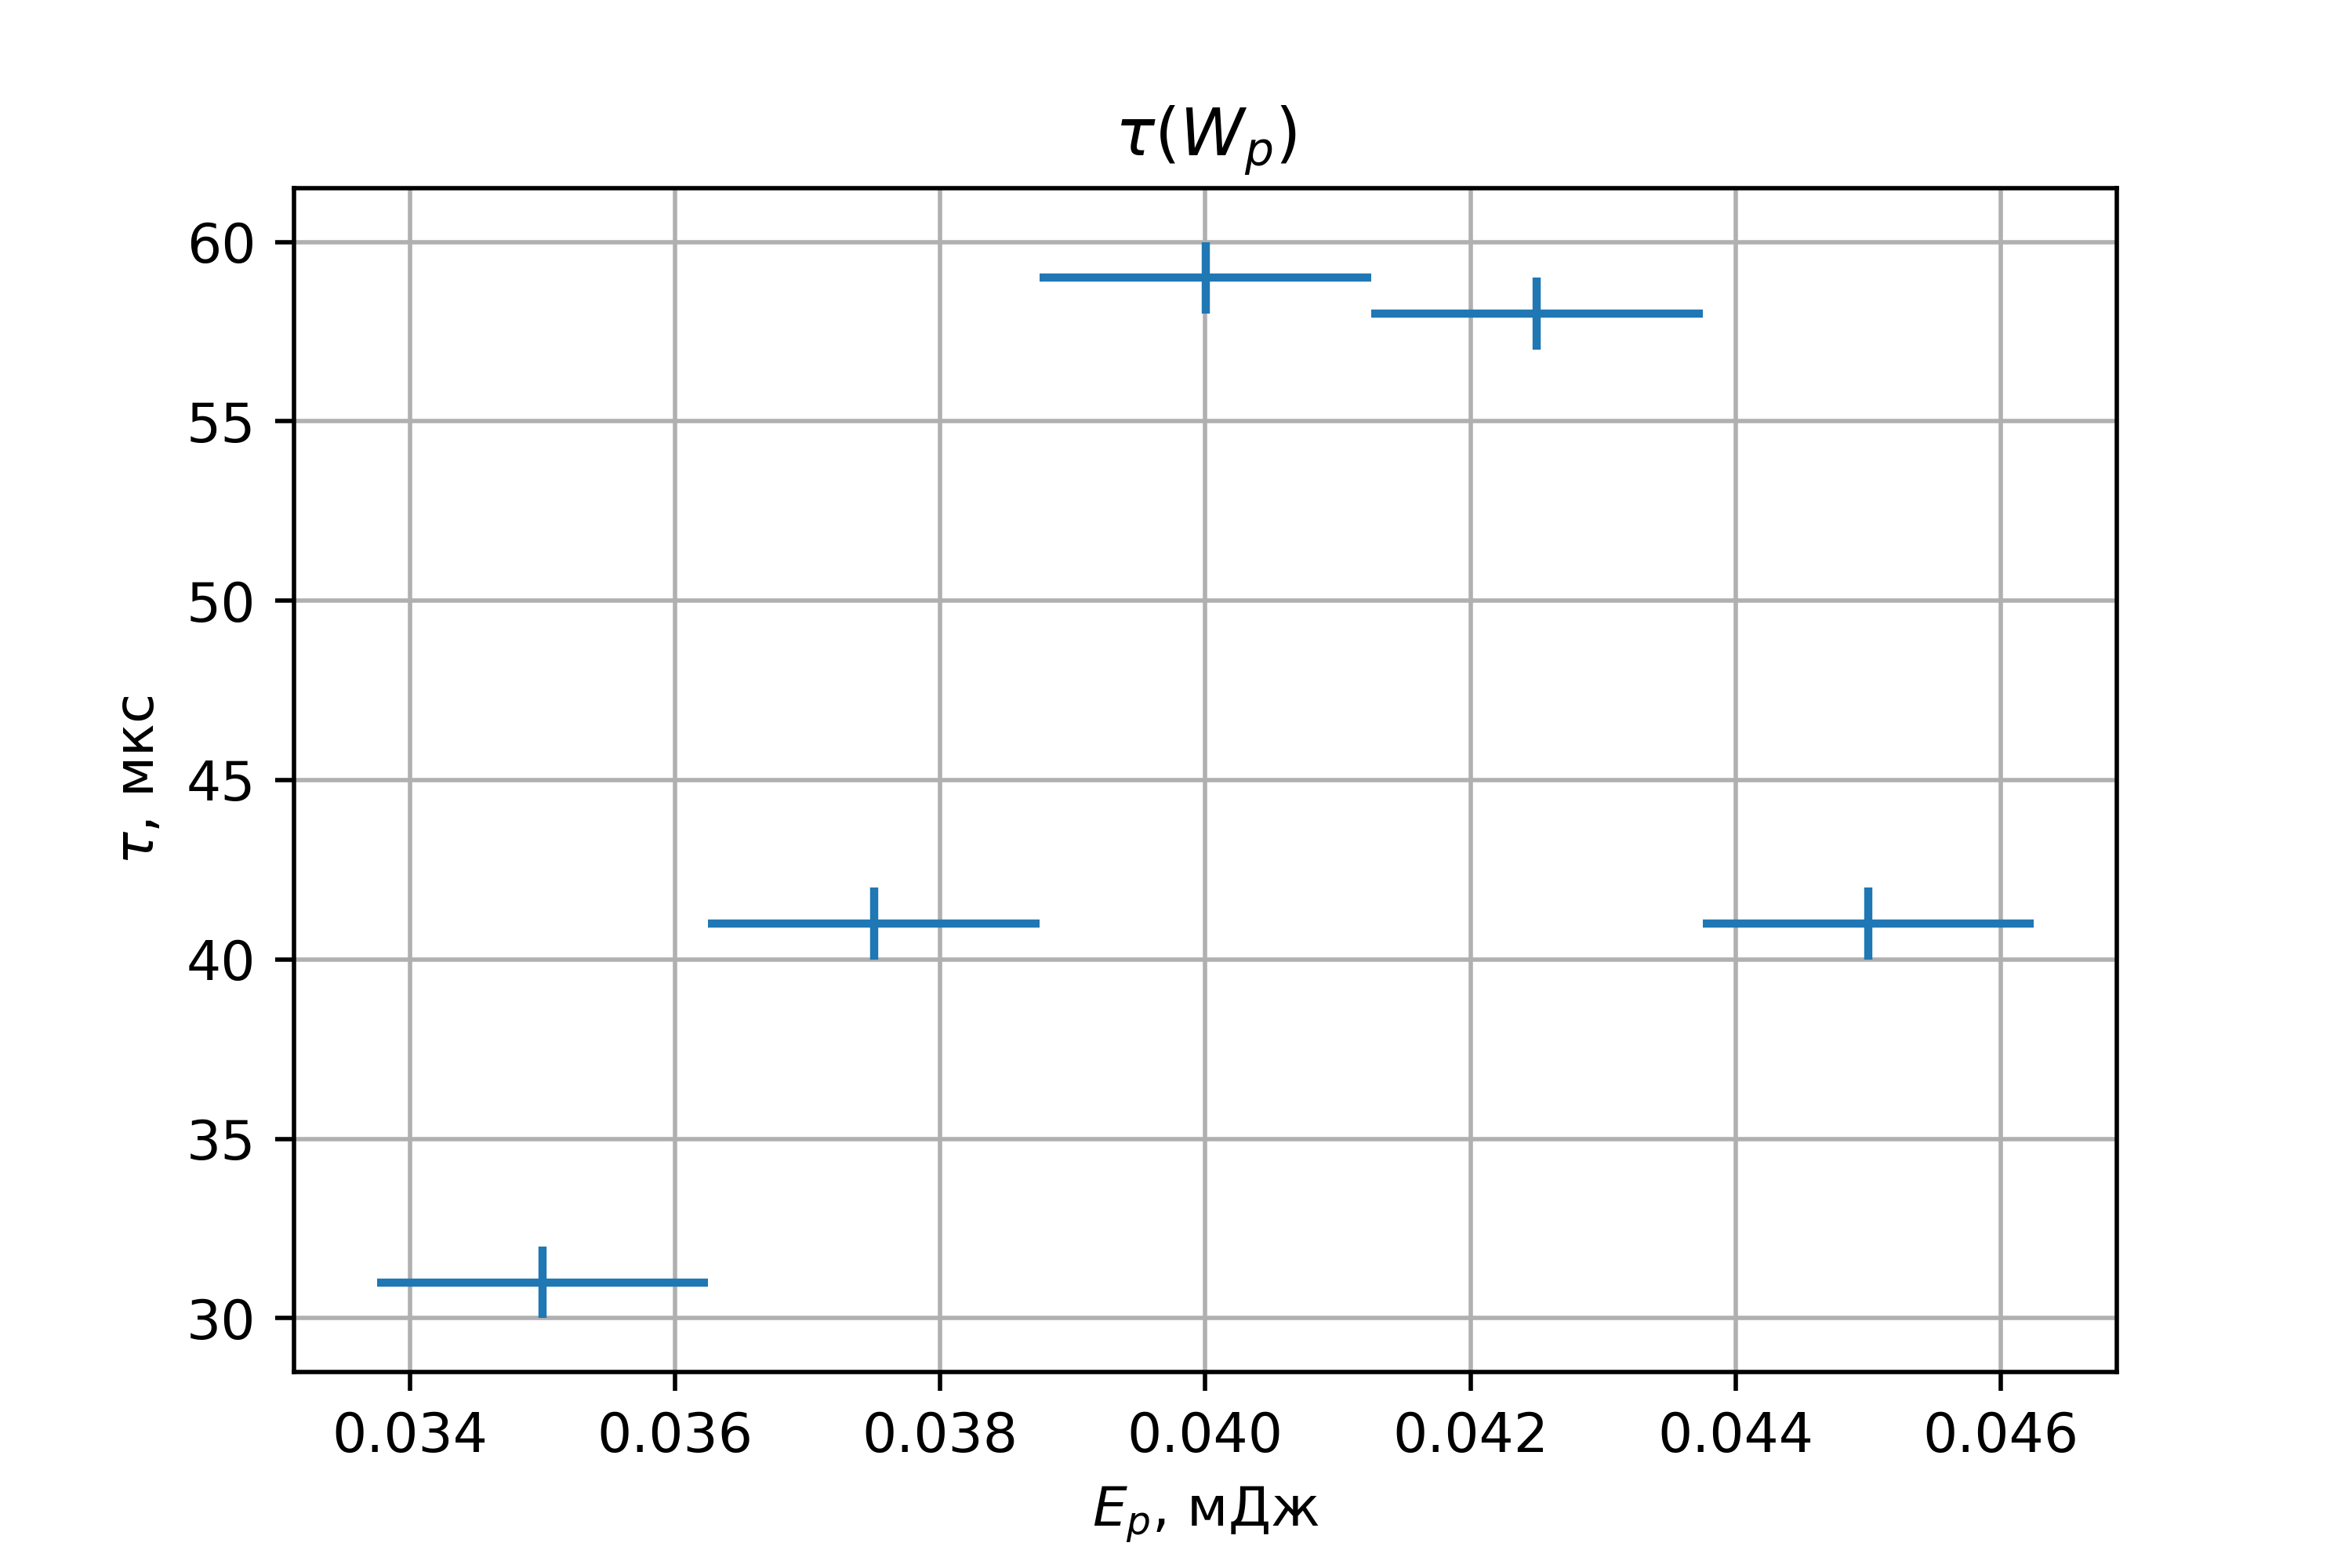
\includegraphics[width=0.65\linewidth]{linear_width2.png}
\caption{Зависимость длительности импульса от энерги накачки}
\label{fig:graph}
\end{figure}


\newpage
\section{Выводы}

\begin{itemize}
	\item Получены КПД и порог генерации в режиме непрерывной генерации
	\item Получены КПД и порог генерации в режиме модулияции добротности
	\item Ширина импульса предположительно не зависит от энергии накачки (или зависит, но не монотонно)
\end{itemize}

\newpage

\section{Задачи}

\begin{itemize}

	\item[1.] Определить необх. инверс. нассел. активных центров ($N=n_2-n_1$), при $R_1,\;R_2,\;\chi_2,\;\langle \chi_1 \rangle,\; \sigma$. \par
		Закон Бугера: \par 
		$$dS_{\omega} = (\chi_1(z) - \chi_2) S_{\omega} (z) dz$$
		Излучение за 1 период: $e^{(\sigma(n_2-n_1)-\chi_2)L}$ \par 
		$$R_1R_2 e^{2L(c} = 1$$
		Условие стационарной генерации: \par 
		$$R_1R_2 e^{2L\sigma(n_2-n_1)-\chi_2} = 1$$

	\item[2.] Доля генерируемой за 2-ой проход в акт. среде свет. мощности. $R_1,\;R_2,\;L,\;\chi_2$ \par 
		Закон Бугера: \par 
		$$dS_{\omega} = (\chi_1(z) - \chi_2) S_{\omega} (z) dz$$
		$$\ln{\frac{S(L)}{S(0)}} = \int_0^L (\chi_1(z) - \chi_2) dz$$
		Пусть $\chi_1(z) \approx \langle \chi_1 \rangle$, где $T = e^{L(\langle \chi_1 \rangle - \chi_2)}$ \par 
		После отражения от правого зеркала: $TS(0)R$ \par 
		После отражения от левого зеркала: $T^2 S(0) R_1R_2$\par 
		$$S(0) = S(0) T^2 R_1R_2$$
		$$e^{2L(\langle \chi_1 \rangle - \chi_2)} R_1R_2 = 1$$
		$$\langle \chi_1 \rangle = \chi_2 + \frac{1}{2L} \ln{\frac{1}{R_1R_2}}$$ Получили сразу в виде лазерного излучения.

	\item[3.] Определить зависимость инверсной заселенности ($n_3-n_2$) в зависимости от плотности фотонов накачки $\rho(\nu_{14})$, 
		где $\nu_{14} = \frac{E_4 - E_1}{\hbar}$. \par 
		Из скоростных уравнений:  \par 
		\begin{equation}
			\begin{cases}
				\frac{n_1}{dt} = -w_{41}(n_1-n_4) + w_{21}n_2 + w_{41}n_4 \\
				\frac{n_2}{dt} = -w_{32}(n_3-n_2) + w_{32}n_3 + w_{21}n_2 \\
				\frac{n_3}{dt} = -w_{32}(n_3-n_2) + w_{43}n_4 + w_{32}n_3 \\
				\frac{n_4}{dt} = -w_{14}(n_1-n_4) + w_{41}n_4 + w_{43}n_4 \\
			\end{cases}
		\end{equation}
		На ур-х 2 и 4 почти нет частиц, тк они быстро переходят на уровни 1 и 4, следовательно $n = n_1 + n_2 + n_3 + n_4 = n_1 + n_3$. \par 
		Приравнивая каждое из уравнений системы к нулю (стационарный режим) получим: 
		\begin{center}
			\fbox{$n_3 - n_2 = n \frac{w_{43}}{w_{32}} \frac{w_{21} - w_{32}}{w_{32} + w_{32}} \cdot \frac{w_{14}}{w_{14} (2 + \frac{w_{43}}{w_{32}}) + w_{14} - w_{43}}$}
		\end{center}

	\item[4.] Возможно ли создание инверсной населенности в 2-ч уровневой схеме в нестационарном случае в приближении балансных уравнений? Определит при заданной мощности накачки $B_{12} \rho$ 
		время $\tau$, через которое $N_1/N_2 = e$. \par 
		Скоростные уравнения: 

		\begin{equation}
			\begin{cases}
				\frac{dN_1}{dt} = w_{21}(N_2-N_1) + w_{21}N_2, & w_{21} = A_{21} \\
				\frac{dN_2}{dt} = - w_{21}N_2 - w_{21}(N_2-N_1), & w_{21} = B_{21}\rho \\
			\end{cases}
		\end{equation}

		\begin{equation}
			\begin{cases}
				\frac{dN_1}{dt} = N_2(A_{21} + B_{21} \rho) - B_{21}\rho N_1 ,& \text{нестац}\\
				\frac{dN_2}{dt} = -N_2(A_{21} + B_{21} \rho) + B_{21}\rho N_1, & \text{нестац}\\
			\end{cases}
		\end{equation}

		$$\det{(A-\lambda E)} = 0\; \Rightarrow \lambda_1 = - A_{21} - 2 B_{21}\rho,\; \lambda_2 = 0$$
		$$\Rightarrow \binom{N_1}{N_2} = C_1 \binom{A_{21} + B_{21} \rho}{B_{21}\rho} + C_2 e^{-(A_{21} + 2B_{21} \rho)t} \binom{1}{-1} $$
		При $t=0,\; N_1=N,\; N_2=0\; \Rightarrow C_1 = \frac{N}{A_{21} + 2B_{21}\rho},\; C_2 = \frac{NB_{21}\rho}{A_{21} + 2B_{21}\rho}$. \par 
		Условие инв. зас. $N_2 > N_1:$ \par 
		\begin{center}
			\fbox{$0 > A_{21}+2B_{21}\rho e^{(...)t} \Rightarrow \; \text{Невозвомжно}$}
		\end{center}
		\begin{center}
			\fbox{$\tau = -\frac{\ln{\left( 1- \frac{A_{21} + 2B_{21}\rho}{B_{21} \rho (e+1)} \right)}}{A_{21} + 2 B_{21}\rho}$}
		\end{center}

	\item[5.] Пусть соотношение населенностей $N_1/N_2 = e$ в термодинамическом равновесии при $T=300K$. ВЫчислить частоту и длину волны излучения перезода. Какая область спектра? \par 
		$$\frac{N_2}{N_1} = e^{-\frac{\hbar \omega}{kT}} = 1/e \Rightarrow \hbar \omega = kT$$
		$$\omega = \frac{kT}{\hbar} \approx 3.9 \cdot 10^{13}\; c^{-1}$$
		\begin{center}
			\fbox{
				$\lambda \approx 48 \; \text{мкм} \; - \text{ИК диапазон}$
			}
		\end{center}

	\item[6.] Какова должна быть температура кристалла АИГ:$Nd^{3+}$ чтобы можно было считать, что лазер работает по трехуровневой схеме? \par 
		\begin{figure}[H]
			\begin{center}
				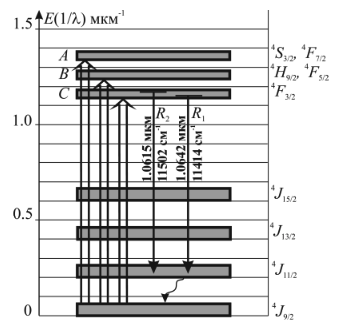
\includegraphics[scale=0.5]{sc1.png}
				\caption{Схема энергетических уровней ионов в кристалле ИАГ.}
				\label{sc1}
			\end{center}
		\end{figure}
		Если верхние 3 уровня склеются $\Delta E \sim 0.2 \; \text{мкм} = kT$ \par 
		$0.2 \frac{1}{\text{мкм}} \approx 4 \cdot 10^{-20} \; \text{Дж} \Rightarrow $
		\begin{center}
			\fbox{$T = \frac{4 \cdot 10^{-20}}{1.38 \cdot 10^{-23}} \approx 2900K$}
		\end{center}

	\item[7.] Найти кол-во продольных мод лазера АИГ:$Nd^{3+}$, $L = 1$м, $\delta \nu =  190$ ГГц. \par 
		Резонансные частоты: $\nu_q = q \frac{c}{2Ln}$. $\lambda = 1.064$ нм, $n = 1.12$ и $\nu_q \approx 1.5 \cdot 10^8$.\par 
		Кол-во мод: 1200.

	\item[8.] Связь между коэффициентами спонтанного и вынужденного переходов Эйнштейна. \par 		
		Ф-ла Планка $\rho_{\nu} = \frac{8 \pi \nu^2}{c^3} \frac{h \nu}{e^{\frac{h \nu}{kT}-1}} $
		Поместили вещество полость АЧТ. Стенки АЧТ при температуре Т. Происходят процессы спонтанного и вынужденного излучений и процессов поглощения.
		Система в теродинамическом равновесии, значит, что число переходов уравновешено. $w_{21} = w_{12} = B_{12} \rho_{\nu}$ 
		$$\Rightarrow AN_{2} + B_{21}\rho N_2 = B_{12}\rho_{\nu}N_1$$
		$$\Rightarrow \rho_{\nu} = \frac{A}{B_{12} e^{\frac{h \nu}{kT}} - B_{21}}$$
		$$\Rightarrow \frac{A}{B} = \frac{8 \pi h \nu^3}{c^3}$$

	\item[9.] Условие генерации в лазере и виды потерь. \par 
		Условие стационарной генерации: $R_1R_2 e^{2L\sigma(n_2-n_1)-\chi_2} = 1$ \par 
		Потери: 
		\begin{itemize}
			\item Потери от зеркал
			\item Рассеяние на излучательных центрах
			\item Возбуждение излучательных центров
		\end{itemize}

	\item[10.] Принципы работы методов модуляции добротности. \par 
		\begin{enumerate}
			\item Пассивная \par 
				Просветляющиеся фильтры, $\Delta E = \hbar \omega$, резонансное поглощение, $n_1<n_2\; \rightarrow$ просветление.
			\item Оптико-механический  \par 
				Вращение одного из зеркал вокруг оси. \par 
				+ простые, недорогие, для любой длины волны \par 
				- шумные, медленная модуляция добротности.
			\item Акустооптический \par 
				Изменение $n$ при распространении ултразвука в среде. Прозрачные материалы с большими значениеми
				акустооптических постоянных. \par 
				+ мало потерь, могут работать в импульсном режиме \par 
				- медленная модуляция добротности.
			\item Электрооптический \par 
				Эффект Поккельса - двойное лучепреломление при наложении постоянного/переменного эл.поля. \par 
				Линейно по полю. $E_x,\; E_y$ - разложение луча, пад. под углом 45$^{\circ}$ на XY плоскость. \par 
				$\Delta \varphi = k L \Delta n, \; \Delta n = n_x - n_y$. $\Delta \varphi= \pi/2 \rightarrow $ поляризация по кругу. После зеркала будет $\Delta \varphi = \pi$. Таким образом,
				линейная поляризация по перпендикулярной изначальной траектории не пройдет через поляризатор.
		\end{enumerate}

	\item[11.] Наиболее эффективный режим (модул. добр, свободная генерация)? \par 
		Эффективность лазера выше в свободной генерации, тк в режиме модуляции добротности существенная часть времени тратится на рост импульса в условии высоких потерь.

	\item[12.] Какова роль резонатора в лазере? \par 
		Положительная обратная связь, селекция на частоте.

	\item[13.] Вычислить величину максимальной спектральной плотности излучения АЧТ, соотв частоту и длину волны излучения при температуре жидкого Гелия, 	
		комнатной и при температуре солнца. Определить степень монохроматичности этого излучения по уровню 0.5, 1/е, 0.1. \par 
		\begin{itemize}
			\item  Закон смещения Вина: $\lambda_{max} = 247 GHz \rightarrow \lambda_{max} = 1.21$ мм. $\rho_{max} = 5.8 \cdot 10^{-25} \frac{\text{Дж}}{m^3 Hz}$ \par 
			\begin{center}
				\begin{tabular}{c|c}
					уровень & $\frac{\Delta \nu}{\nu_{max}} $ \\ \hline
					0.5 & 1.5 \\ 
					1/e & 1.8 \\ 
					0.1 & 2.8 \\ 
				\end{tabular}
			\end{center}
				
			\item Комнатная $T=300K,\; \nu_{max} = 17.6 THz \rightarrow \lambda_{max} = 17$ мкм. $\rho_{max} = 2.1\cdot 10^{-10} \frac{\text{Дж}}{m^3 Hz}$ \par 
			\begin{center}
				\begin{tabular}{c|c}
					уровень & $\frac{\Delta \nu}{\nu_{max}} $ \\ \hline
					0.5 & 1.5 \\ 
					1/e & 1.8 \\ 
					0.1 & 2.8 \\ 
				\end{tabular}
			\end{center}

			\item Солнце $T=5780K$. $\nu_{max} = 330.8 THz \rightarrow \lambda_{max} = 883$ мм. $\rho_{max} = 1.5\cdot 10^{-15} \frac{\text{Дж}}{m^3 Hz}$ \par 
			\begin{center}
				\begin{tabular}{c|c}
					уровень & $\frac{\Delta \nu}{\nu_{max}} $ \\ \hline
					0.5 & 1.5 \\ 
					1/e & 1.8 \\ 
					0.1 & 2.8 \\ 
				\end{tabular}
			\end{center}
		\end{itemize}
		
	\item[14.] Сравнить вероятности индуцированных переходов в единицу времени под действием излучения АЧТ с температурой солнца и излучения стандартного гелий-неонового лазера. \par 
		Нужно понять какая спектр. плотность излучения у лазера. Она будет определяться плотностью энергии в обьеме выходящего из лазера луча.

	\item[15.] Определить температуру, при которой сравниваются между собой  вероятности спонтанных и индуцированных переходов в единицу времени для рентгеновского, ультрафиолетового, инфракрасного, миллиметрового диапазовнов. \par 
		Вер. спонтанного перехода = вер. индуцированных переходов. \par 
		$$B = \frac{\pi^2 c^3}{\pi \omega^3} A$$
		$$\rho = \frac{8 \pi \nu^2}{c^3} \frac{h \nu}{e^{\frac{h \nu}{kT} - 1}}$$
		$$\frac{c^3}{8 \pi h \nu^3} \left( \frac{8 \pi \nu^2}{c^3} \frac{h \nu}{e^{\frac{h \nu}{kT} - 1}} \right) = 1$$

		\begin{center}
			\begin{tabular}{c|c|c}
				\hline
				рентген & 1 А & $2 \cdot 10^8 K$ \\ 
				УФ & 100 нм & $2 \cdot 10^5 K$ \\ 
				ИК & 10 мкм & $200K$ \\ 
				мм & 1 мм & $20K$ \\ 
			\end{tabular}
		\end{center}

	\item[16.] Рассчитать спектральную ширину резонанса и добротность "холодного" резонатора, если длинна резонатора $L=90$ см, а коэффициенты отражения зеркал $R_1=R_2=98$. \par 
		$Q = 2 \pi \nu \tau_c = -2 \pi \frac{c}{\lambda} \frac{2 L}{c \ln{R_1R_2}} = -\frac{4 \pi L}{\lambda \ln{R_1R_2}} \approx 2.6 \cdot 10^8$ \par 
		$\Delta \omega = -\frac{c \ln{R_1R_2}}{2 L} = 6.7 \cdot 10^6$ рад/с.

	\item[17.] Рассчитать пороговую инверсию и пороговую мощность накачки для лазера, используемого в работе, $R_1=100\%,\; R_2=50$. \par 
		Порог генерации $R_1R_2 e^{2 \sigma (n_2-n_1)L} = 1$ \par 
		Порог инверсии $n_2-n_1 = - \frac{\ln{R_1R_2}}{2 L} = 1.1 \cdot 10^{16}\; 1/cm^3$
	
\end{itemize}





\end{document}